\Chapter{A kérdésgeneráló webalkalmazás megvalósítása}

Ezen fejezet célja az általam készített kérdésgeneráló mintaalkalmazás bemutatása. Terítékre kerül az alkalmazás célkitűzése, tervezése, fejlesztési menete, végül pedig az alkalmazás tesztelése, mind automatikus, mind pedig manuális formában. Kitérek továbbá a felhasznált programozási eszköztárak bemutatására, azok előnyeivel és hátrányaival együtt.

\Section{Az alkalmazás célja}

Ez a webalkalmazás a dolgozatomban bemutatott módszerek gyakorlati alkalmazásának bemutatására szolgál. Az alkalmazás alapvetően egy online kérdésgenerátor, melynek meg lehet adni egy szöveges kontextust és az alapján a program mögött álló modell generál bizonyos számú kérdést. A célom az volt, hogy biztosítsak egy nagyon egyszerű, átlátható és jól kezelhető interfészt, továbbá hogy maga az algoritmus is minél relevánsabb kérdéseket alkosson meg. Mindezt online formában képzeltem el, hiszen az alkalmazás szerver oldali(backend) része meglehetősen erőforrás-igényes, így azt egy egyszerű asztali alkalmazás formájában nehéz lenne futtatni, illetve így bárhonnan szabadon elérhetővé válik a program.

\Section{A programmal szemben támasztott \\ követelmények}

\begin{itemize}
\item \textbf{Gyors válaszidő, optimális működés}: Mivel az alkalmazás mögött egy nagyobb neurális hálózat van, így mindenképp biztosítani kell, hogy a szerver rendelkezzen a megfelelő mennyiségű memóriával, processzormaggal vagy akár videokártyával, annak érdekében, hogy reális válaszidőket kapjon a felhasználó. Továbbá a kódnak is alkalmazkodnia kell a körülményekhez, így rövidnek, átláthatónak és gyorsnak kell lennie.
\item \textbf{Letisztult felhasználói interfész}: Az alkalmazás alapvető céljából fakadóan biztosítani kell az egyszerű kezelhetőséget. Alkalmasnak kell lennie tetszőleges méretű szöveges kontextus feldolgozására, illetve a generált kérdéseknél is törekedni kell a könnyű másolhatóságra, hogy a felhasználó később be tudja illeszteni dokumentumaiba őket.
\item \textbf{Megfelelő minőségű kérdések}: Az alkalmazás által kreált kérdések nem térhetnek el a megadott kontextustól, de törekedni kell arra, hogy ne csak a megadott szövegből kimásolva kérdezzen, hanem érződjön valamilyen háttértudás is a kérdések mögött. Illetve a kérdéseknek az adott nyelven értelmesnek kell lenniük.
\item \textbf{Általános tudásbázis}: Szükség van arra, hogy az alkalmazás minél több témakörből képes legyen kérdéseket generálni, így olyan tanítóhalmazra van szükség, ami nem korlátozódik egyetlen témára, illetve több kérdés típust is tartalmaz.
\end{itemize}

\Section{A program megtervezése}

Az alkalmazás elkészítését hosszas tervezőfolyamat előzte meg. Első lépésként választani kellett egy megközelítési módot az alapfeladat megvalósításához. Számos módszertan létezik a kérdésgeneráláshoz, de végül a neurális hálózat alapú megoldás mellett döntöttünk, azon belül is a már részben előtanított transformer modellek mellett, melyek már rendelkeznek alapvető háttértudással, így már csak a kérdésgenerálás megvalósítására kell megtanítani őket.

Következő lépésként el kellett dönteni, hogy milyen nyelven történjen a kérdésgenerálás. Itt szükséges volt összeszedni, hogy az egyes nyelveken milyen mennyiségben áll rendelkezésre tanítóhalmaz a neurális hálózat tanításához, hiszen elengedhetetlen, hogy a hálózat lásson kontextusokat és hozzájuk készült kérdéseket mintának, ami alapján később képes lesz saját magától is hasonló kérdéseket alkotni. Végül az angol nyelvre esett a választás, mert ezen a nyelven találtunk megfelelő tanítóhalmazt és a feladathoz illő alaptudással rendelkező hálózatot, melyet később tovább tudtunk tanítani.

Ezután a megfelelő transformer hálózat kiválasztása következett. Számos modellt megvizsgáltunk az alapján, hogy:

\begin{itemize}
	\item Mennyire megoldható rajta feladatunk?
	\item Mennyire optimális a működése?
	\item Tudjuk-e saját gépen vagy egyéb szerveren futtatni, tárolni és tanítani?
	\item Mekkora a mérete?
	\item Kellően fejlett-e a feladat megoldásához?
	\item Ingyenesen elérhető-e és lehet-e tovább tanítani?
\end{itemize}

Először a BERT modellt vizsgáltuk. Számos kutatást és cikket találtunk a témában, melyek sikeresen alkalmazták a BERT-et több NLP feladatra. Kérdésgenerálásra is alkalmazhatónak tűnt, azonban a tanítása nehézkesnek bizonyult, illetve nagyon hamar találtunk sokkal jobb és kifejezetten szöveggenerálásra használható modelleket, melyek könnyebben kezelhetők, gyorsabbak és jobb eredményeket is produkáltak.

A GPT-2 nevű modell már ígéretesebbnek tűnt, hiszen kifejezetten szöveggenerálásra hozták létre és kb. 40 GB szöveges adattal tanították be, ami már jelentős eredménynek számított a területen. Ingyenesen elérhető és letölthető, valamint szabadon lehet tovább tanítani is. Szöveggenerálási eredményei elég jók voltak és számos kutatást találtunk, ahol kérdés megválaszolásra és kérdés generálásra tanítják, de más modellekkel összehasonlítva nem ezt találtuk a legjobbnak.

A GPT-3 modell minden szempontból túlszárnyalta elődjét. Amellett, hogy a hálózat architektúráját átszervezték, jelentősen növelték a tanulási paramétereinek számát és a tanítási adathalmaz méretét is, így rendkívül jó eredményeket produkál szinte az összes NLP feladat esetén, így a kérdésgenerálásban is. Egyetlen hátránya a modellnek a mi szempontunkból, hogy csak korlátozottan használható és jelenleg nem ingyenes a hozzáférése.

Számunkra a legmegfelelőbb modellnek a Google T5 nevezetű modellje bizonyult, ami már kifejezetten fejlett, kiválóan alkalmazható mindenféle szöveggenerálási feladatra és nagyon könnyen betanítható kérdésgenerálásra, amellett, hogy meglehetősen kedvező méretű. A Hugging Face nevű oldalon ingyenesen elérhető módon meg is található betanított változatban, melyet tovább tanítva megoldhattuk feladatunkat.

Mivel az alkalmazás céljai között szerepel, hogy online elérhető legyen, így ezután elkezdődhetett a szerveroldali működés kidolgozása. A szerver programozási nyelvénél a Python-ra esett a választás, mivel nagyon hasznos könyvtárai vannak adatelemzés és statisztika területén, illetve webfejlesztési területen elérhető hozzá egy Django nevű szerveroldali keretrendszer is, mely jelentősen megkönnyítette a szerver elkészítését. Magának a szervernek egyetlen főbb végpontot kellet biztosítani, ami a megadott szöveges kontextust fogadja és válaszként visszaadja az elkészült kérdéseket. Miután az alkalmazás nem tárol felhasználói adatokat, így adatbázisszerver nem lett konfigurálva hozzá, de a rendszer úgy lett kialakítva, hogy ha idővel mégis szükség lenne rá, akkor könnyen be lehet csatlakoztatni egy tetszőleges adatbázist. 

Mindezek mellett szükségessé vált időközben, hogy magának a neurális hálózatnak a tanítását és működését valamilyen szinten szeparáljuk a szervertől, hiszen ez a feladatrész akár napokig is eltarthat még erősebb hardver esetén is. Ezért született az a döntés, hogy a tanításért felelős kódokat vegyük külön egy önmagában futtatható kódfájlba, melyet bárhol képesek vagyunk futtatni, például valamilyen felhőszolgáltatáson és utána a betanított hálózatot, ha van rá lehetőség mentsük el egy tárhelyre, majd onnan a szerver töltse be és már készen, előtanítva használja azt. A tanításért felelős felhőszolgáltatásnak a Google Colab nevű rendszerét használtuk, míg a betanított hálózatot a Hugging Face nevű oldalon tároltuk el, ahonnan egy egyszerű API-n keresztül könnyen le is tudtuk tölteni saját szerverünkre, ahol egyszerű fájlként tud tárolódni.

Miután megterveztük a szervert következhetett a kliensoldali(frontend) rész. Itt a Vue.js nevű frontend keretrendszert választottuk, mivel kisméretű, gyors és könnyű benne a fejlesztés is. A rendszer komponensalapú megközelítése segítette az alkalmazás egyszerű és átlátható működésének biztosítását. Az klienshez igyekeztünk letisztult dizájnt választani, melyen egyértelmű minden funkció és biztosított, hogy a felhasználó a program minden funkciójának tudja a szerepét. Szempont volt például, hogy tetszőleges méretű kontextust tudjon kezelni a kliens, illetve, hogy a kérdések együtt és külön-külön is kimásolhatóak legyenek a későbbi felhasználásukhoz. A felületen történő navigációt pedig ikonok és apró súgószövegek segítik.

Az utolsó lépés a tesztek és tesztesetek előkészítése volt. A jelenlegi és jövőbeli fejlesztés megkönnyítése érdekében szükséges volt automatizált teszteket készíteni, mint például egységteszteket és integrációs teszteket. Mindezeket kliens és szerveroldalon is el kellett készíteni. Továbbá, mivel egy NLP feladatot oldunk meg, így szükségessé vált a manuális, kézi tesztelés is különböző tesztesetekkel. Elsőkörben természetesen az alap eseteket kellett vizsgálni, hogy egyáltalán értelmes kérdések készülnek-e, majd pedig következhettek a komplexebb szituációkat bemutató tesztek.

\Section{Telepítés és futtatás}

Mivel alkalmazásunk alapvetően webes környezetbe lett szánva, így lokális futtatása nem feltétlenül egyszerű feladat, de azért törekedtünk a könnyű elindítás biztosítására. Ennek érdekében elérhetővé tettük az alkalmazást Docker környezetben. A Docker használatához mindössze a Docker Desktop nevű alkalmazás telepítése szükséges, amely elérhető Windows, Linux és MacOS operációs rendszereken is. Ekkor a frontend és backend rész együttes futtatása mellet a http://localhost:3000 cím alatt válik elérhetővé az alkalmazás.

Azonban a tesztelés megkönnyítése végett éles környezetben is elérhetővé tettük a webalkalmazást a következő URL alatt:

\vspace{1cm}

\centerline{\url{https://mb-thesis-t5-qg-frontend-oumla56ewq-lm.a.run.app}}

\vspace{1cm}

Az éles környezetet a Google Cloud biztosítja számunkra, ahol bizonyos mennyiségű havi szerver felé indított kérésig ingyenesen biztosítanak nekünk lehetőséget alkalmazásunk tárolására. A nap első indításánál lassabb lehet az oldal betöltése, de általában gyorsan el lehet érni a weboldalt és a kérdésgenerálás se tart túl sokáig a biztosított hardvereken.

Az alkalmazás lokális elindításához elengedhetetlen néhány alapkövetelmény, melyeknek rendszerünknek meg kell felelnie:

\begin{itemize}
\item Hardverek tekintetében bár igyekeztünk tehermentesíteni az alkalmazást a szeparált tanítókomponensekkel, de a szervernek így is jelentősebb memória és processzor igénye van. Ajánlott legalább 16GB memória és egy 4 magos processzor, illetve 5 GB szabad hely a lemezen.
\item A szerver az első indítás alkalmával letölti a betanított transformer hálózat aktuális verzióját, így az első indításhoz mindenképp szükséges hálózati kapcsolat.
\item Operációs rendszerek tekintetében alapvetően nincs megkötés. Szimplán csak működjön az adott rendszeren a Docker Desktop alkalmazás és engedje a virtualizációt valamilyen formában.
\item A telepítés során ajánlott a haladó szintű felhasználói ismeret(jegyzék struktúrák, terminál ismerete stb.)
\item Az alkalmazást Google Chrome, Firefox, Opera és Microsoft Edge böngészőkön teszteltük, így a futtatása is onnan ajánlott.
\end{itemize}

Miután meggyőződtünk a fenti követelmények teljesüléséről a következő lépésekkel tudjuk feltelepíteni az alkalmazást:

\begin{itemize}
\item Töltsük le és telepítsük fel a Docker Desktop nevű alkalmazást. Az alkalmazás elérhető a \url{https://www.docker.com/products/docker-desktop} weboldalról Windows, Linux és MacOS rendszerekre is egyaránt. Erre az alkalmazásra a virtualizáció miatt van szükség, ami jelentősen megkönnyíti a telepítést.
\item Lépjünk be terminálon vagy cmd-n keresztül a program mappájába és futtassuk a \textit{docker-compose up} parancsot. Ez a parancs létrehoz egy virtuális konténert külön a szerver és külön a kliens oldali architektúrának.
\item Következő lépésben lépjünk be az alkalmazás \textit{qg\_app\_frontend} mappájába és a \textit{.env.dist} fájl alapján hozzunk létre egy \textit{.env} fájlt.
\item A \textit{.env} fájlban a \textbf{VITE\_BASE\_URL} változó a szerver elérhetősége \\
(pl. \url{http://localhost}), míg a \textbf{VITE\_ENV} a kliens környezetének beállítására szolgál, ami lehet fejlesztői(dev) vagy éles(prod).
\item Ezután elérhetővé válik az alkalmazás kliens oldali része a \url{http://localhost:3000}-es cím alatt, míg a szerver a \url{http://localhost:80}-as cím alatt lesz megtalálható.
\end{itemize}

\Section{Az alkalmazás felhasználói felülete}

\begin{figure}[h]
\centering
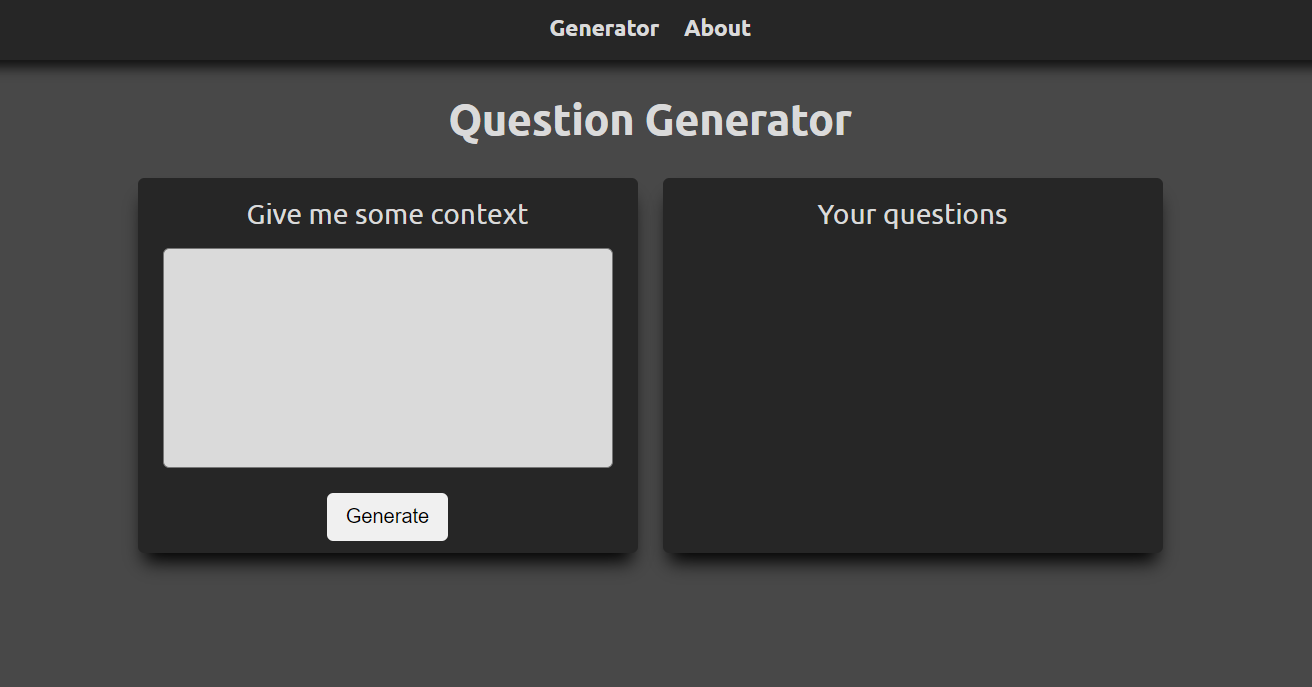
\includegraphics[scale=0.5]{images/app_ui.png}
\caption{A program felhasználói felülete.}
\label{fig:app_ui}
\end{figure}

A program nagyon egyszerű felhasználói interfészt használ. Adott 2 oldal: a főoldal és egy az alkalmazás leírását tartalmazó oldal. A főoldalon található maga a kérdésgeneráló komponens. A komponens bal oldalán lehet megadni a szöveges kontextust, ami alapján a kérdések generálódnak, míg a jobb oldalon fognak megjelenni az elkészült kérdések, könnyen másolható formában.

\begin{figure}[h]
\centering
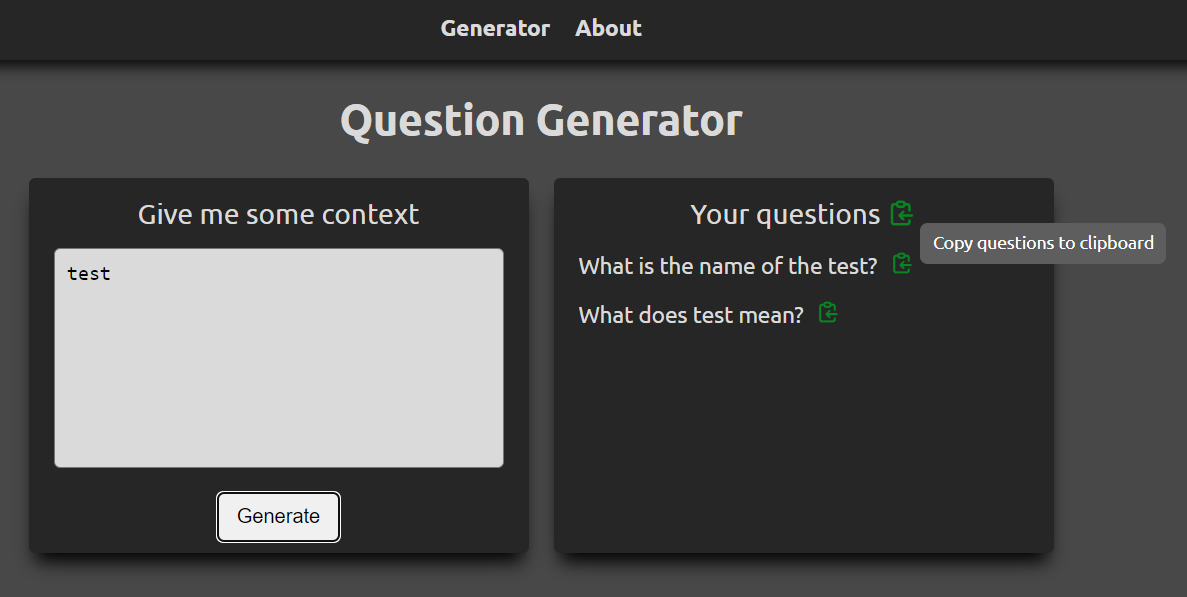
\includegraphics[scale=0.5]{images/app_ui_2.png}
\caption{Az elkészült kérdések.}
\label{fig:app_ui_2}
\end{figure}

\Section{Felhasznált fejlesztői eszközök bemutatása}

Mielőtt bemutatnám az alkalmazás részletes működését, szeretném ismertetni a fontosabb felhasznált, elsősorban szerveroldali programkönyvtárakat(API-kat), melyek jelentősen megkönnyítették a fejlesztést. Ezen könyvtárak szinte mindegyike feltelepíthető a Python alapértelmezett csomagkezelőjével, a \textbf{pip}-el.

\SubSection{datasets}

A \textbf{datasets} könyvtár számos hasznos funkciót tartalmaz különböző adatforrások betöltésére, feldolgozására és megosztására. Nagyon sokan használják az NLP, számítógépes látás, adatfeldolgozás területén. Előnye, hogy képes nagy méretű adatforrásokat gyorsan és optimálisan a memóriában tárolni, ahonnan később felhasználhatjuk azt alkalmazásunkban. Legfontosabb metódusa a \textbf{load\_dataset} metódus, melynek segítségével betölthetjük lokális vagy online formában elérhető adatforrásainkat.

\SubSection{transformers}

Ez a könyvtár felelős az előtanított hálózatok kezeléséért. Lehetőség van letölteni különböző betanított neurális hálózatokat, melyeket később tovább taníthatunk(fine-tuning), illetve fel is tölthetünk a Hugging Face Hub nevű platformra, ahonnan futtathatjuk és meg is oszthatjuk másokkal megoldásainkat. Ez a megközelítése a mesterséges intelligencia alapú hálózatoknak úttörő jelentőségű, hiszen nagyon közel áll az emberi agy működéséhez, melynek működési alapelve a folyamatos tanulás és a különböző  feladatokra való specializálódás.

Az első fontosabb funkció a könyvtárban a \textbf{pipeline} metódus, melynek segítségével különböző feladatokra specializálódott előtanított hálózatokat használhatunk \\
kódunkban\cite{hf}. A metódus meghívásánál egyszerűen csak meg kell neveznünk a kívánt feladatot, választhatunk egy modellt, aminek segítségével fogja megoldani a feladatot, illetve biztosítanunk kell egy paramétert neki, ami a feladattól függően lehet egy kép, hangfájl, szövegrészlet vagy egyéb egyszerűbb értékek is. A metódus eredménye végül egy objektum lesz, mely a megoldásokat tartalmazza és szintén tetszőleges típusú lehet. A végeredmények mellé általában társul valamilyen statisztika is, hogy a modell milyen biztossággal állította elő az adott eredményt.

Egy másik lényeges koncepció a könyvtárban az ún. \textbf{tokenizer}-ek, melyek a modellek bemenetének előkészítésében játszanak jelentős szerepet. Működésük során a bemeneti szövegrészeket különböző egységekre bontják és ellátják őket azonosítókkal, majd pedig az elkészült token-eket kódolják\cite{hf}. Ezt a folyamatot visszafelé is képesek megcsinálni, így tokenekből képesek dekódolni az elkészült szöveges eredményeket. Az alap funkciókon felül saját kódolást és feldolgozási lépéseket is hozzáadhatunk működésükhöz, ezáltal tudjuk feladatunkhoz szabni őket. Az alap tokenizer osztály a \textbf{PreTrainedTokenizerBase}, mely tartalmazza a kódoláshoz, dekódoláshoz, tokenizáláshoz és speciális tokenek definiálásához szükséges funkciókat. Ezt az osztályt kiterjesztve lehet saját tokenizer-t is készíteni.

A modellek tanításához a könyvtár biztosítja a \textbf{Trainer} osztályt. Ez az osztály felel az alap tanítási ciklus elkészítéséért. Támogatja az elosztott, párhuzamos tanítást is grafikus processzoron(GPU), illetve tenzor-feldolgozó egységen(TPU). Argumentumként meg kell adnunk a Trainer-nek a modellünket, amit tanítani szeretnénk, a tanító, illetve validáló adathalmazokat, valamint egy \textbf{DataCollator} osztályt, ami az adathalmazok csoportokra bontásáért felel, így gyorsítva a tanítást. Ezen kívül megadhatunk egy \textbf{TrainingArguments} objektumot neki, ahol beállíthatjuk\cite{hf}:

\begin{itemize}
\item a különböző hardveren való tanítással kapcsolatos attribútumokat
\item a tanulási rátát
\item a tanulási ciklusok számát
\item hány lépésenként mentse el a hálózat aktuális állapotát
\item készítsen-e jelentéseket a hálózat adott pillanataiban a súlyairól és hiba rátájáról
\item elmentse-e lokálisan vagy a Hugging Face Hub nevű oldalra az elkészült hálózatot
\end{itemize}

Az utolsó fontosabb funkciója a könyvtárnak a \textbf{modellek}, melyek a már ténylegesen elkészült, betanított neurális hálózatainkat fogják kezelni. A könyvtár által biztosított \textbf{PreTrainedModel} osztályok tartalmazzák az olyan funkciókat, mint a hálózatok betöltése egy adott lokális vagy online elérhető helyről, a hálózat mentése, illetve a bemeneti tokenek átméretezése a tokenizernek és a hálózatnak megfelelő méretre\cite{hf}. Ezen osztályra épül az általam használt \textbf{T5ForConditionalGeneration} nevű modell osztály is, mely képes eltárolni és kezelni az előtanított T5 modelleket, illetve kompatibilis a \textbf{T5Tokenizer} osztályokkal is, így könnyítve a tanítóhalmazok és a végeredmények feldolgozásán. A T5-höz hasonlóan lehet találni más modell osztályokat is a könyvtárban, például léteznek BERT-hez, GPT-hez és ezek különböző változataihoz készült modellek és tokenizerek is.

\SubSection{torch}

A \textbf{torch} biztosítja számunkra a hardveres gyorsítást. Segítségével tanítóhalmazunkat eltárolhatjuk ún. tenzorokban, melyek lényegében azonos típusú adatokat tartalmazó többdimenziós mátrixok és ezeket felhasználva tudjuk tanítani neurális hálózat modellünket általános processzoron, grafikus processzoron vagy tenzor-feldolgozó egységen. A \textbf{transformers} könyvtár is támogatja a torch-al való hardveres gyorsítás használatát a \textbf{DataCollator} osztályokon keresztül, melyek pont a tanítási adatok csoportosításáért felelnek. A könyvtár használatával jelentősen fel tudtuk gyorsítani a tanítási és szöveggenerálási időket alkalmazásunk esetében is.

\SubSection{SQuAD adathalmaz}

A \textbf{Stanford Question Answering Dataset(SQuAD)\cite{squad}} a Stanford Egyetem által készített szabad hozzáférésű szövegértési adathalmaz. Több mint 100 000 kontextus-kérdés-válasz hármasból áll, melyeket Wikipedia cikkek alapján állítottak össze. Az egyes adatrekordokhoz tartozik egy rövidebb szöveges kontextus, 4-5 kérdés, illetve minden kérdéshez néhány helyes válasz. Az egyes válaszoknál az is meg van adva, hogy a kontextusban hol található meg a válasz(ez inkább a kérdés megválaszolási feladatoknál fontos szempont). Alkalmazásunkban ezt az adathalmazt használtuk a kérdésgeneráló T5 alapú neurális hálózat betanítására. Ehhez egy adatbetöltő szkriptet használtunk, mely csatolva lett a dolgozathoz, illetve a \url{https://huggingface.co/datasets/squad/blob/main/squad.py} URL alatt is elérhető.



\Section{A program részletes működése}

\SubSection{A hálózat tanításáért felelős komponens}

Mint azt már a tervezési részben említettem a tanításért felelős komponensek hardverigényük miatt szeparált fájlba és környezetbe kerültek a program többi részétől annak érdekében, hogy megfelelő és költséghatékony helyen lehessen őket futtatni. Emiatt a hálózat tanítási részét egy Python alapú \textit{.ipynb} fájlba szerveztük, melyet a Google Colab nevű felhőalapú környezetben tudtunk lefuttatni. 

A szükséges könyvtárak importálása után a program kér egy bejelentkezést a Hugging Face Hub nevű platformra, melyre később a már betanított hálózatot fogja menteni, illetve kéri az adathalmazt is, mely esetünkben a csatolt \textit{t5\_squad.py} fájl lesz, ami a SQuAD adathalmazt fogja letölteni és megfelelő formátumra alakítani a későbbi feldolgozáshoz.

A következő lépés az adatok előfeldolgozása. Itt már szükséges volt definiálnunk az alap transformer modellünket, ami a \textit{t5-base} lesz, mert az előfeldolgozáshoz szükségünk van egy tokenizer-re, melynek mérete meg kell egyezzen a modell bemeneti token mátrixának méretével, így ezt itt be kell állítanunk. Ezután következhet a nyers adathalmaz tokenekre bontása és kódolása, melyet az alap modellhez tartozó tokenizer segítségével végezhetünk el. A fázis kimenete egy tanítási és egy validációs adathalmaz lesz, melyet a hálózat tanítása során fogunk tudni majd felhasználni.

Miután elkészült a tokenizált és kódolt bemenet, elkezdhetjük a hálózat tanítását. A \textit{torch} könyvtár tenzorai segítségével különböző csoportokra bontjuk a bemenetet egy \textit{DataCollator} osztályban, így lehetővé téve a GPU-n vagy TPU-n való párhuzamosítást. A \textit{Trainer} osztály segítségével és néhány argumentum megadása után végül elindíthatjuk a tanítást. A trainer jelenleg 4-es csoportokban képes az egyes GPU/TPU magokon tanítani a hálózatot, 100 lépésenként jelentést készít, illetve 500 lépésenként menti is a hálózat aktuális állapotát. Természetesen erősebb hardvereken meg lehet próbálni nagyobb csoportokban tanítani a hálózatot, de gyengébb hardvereken gyakran futhatunk ki a memóriából a nagyobb csoportszám miatt.

Utolsó lépésben a szkript feltölti a Hugging Face Hub nevű platformra a hálózatot, ahonnan később a szerverünk letöltheti és használhatja azt.

\SubSection{Szerveroldali komponens}

Az alkalmazás szerveroldali nyelve a tanító komponenshez hasonlóan Python, mivel így sokkal egyszerűbben tudtuk kezelni a neurális hálózatot. A szerver Django keretrendszer segítségével lett elkészítve, mely biztosítja számunkra a könnyű és gyors futtatást és az eszköztárakat. A szerver konfigurációját tekintve nyílt, így lényegében bármely alkalmazás elérheti az interneten keresztül. Jelenleg adatbázist nem tartalmaz a szerver, így felhasználói és egyéb alkalmazás adatok nem kerülnek tárolásra a futás során.

Szerveroldalon az egyetlen végpont, amit implementálnunk kellett az a \\
\textit{api/generate-questions} nevű útvonal. Ez felel majd a megadott kontextushoz generált kérdések elkészítéséért. A \textit{transformers} könyvtárt itt is telepíteni kellett, hiszen szükségünk van a tokenizer-ünkre és a modellünkre a kérdések generálásához. A tokenizer és a modell definiálása után a megadott szöveges kontextust a tokenizer segítségével kódoljuk és átadjuk a modellünknek, hogy generáljon ez alapján kérdéseket. A generáláshoz, akár csak a modell tanításához számos paramétert adhatunk meg. Változtathatjuk a maximálisan kigenerálható kérdések mennyiségét, a kérdések hosszát, az egyes szavak maximális ismétlődését, illetve a dekódolási algoritmust is beállíthatjuk, ami lehet mohó keresés, sugár keresés, top-k mintavétel vagy top-p mintavétel is.

A generált és dekódolt kimeneti kérdéseket végül szöveges tömb formájában adja vissza a szerver, JSON formátumban, amit aztán a kliens fel tud dolgozni.

\SubSection{Kliensoldali komponens}

A kliensoldal TypeScript-ben íródott és a Vue.js nevű frontend keretrendszert használtuk az elkészítéséhez, ami biztosítja a HTML, CSS, és JavaScript kódok összecsomagolását, optimalizálást, illetve a kódolást is jelentősen megkönnyíti. A kliensoldali működés oldalakra és komponensekre lett bontva. Két oldalt használ az alkalmazás: a főoldalt, ahol a kérdésgenerátor van, valamint egy leírás oldalt, ahol az alkalmazás használata és bemutatása van részletezve.

Komponensek közül a \textit{QuestionGenerator} a legfontosabb, amely magát a kérdésgenerálás kliensoldali részét tartalmazza. Itt adott egy szövegdoboz, amibe a felhasználó beírhatja a szöveges kontextust, ami alapján szeretne kérdéseket generálni. Ezután a komponens kapcsolatot létesít a szerverrel és sikeres szerverválasz esetén megjeleníti az elkészült kérdéseket. A kérdések ezután egy segédfüggvény segítségével kimásolhatók és szabadon beilleszthetők bármilyen dokumentumba.